% So I have up to 11 texts I need to show here
% lut64
% pext64
% shuffle64
% shuffle128
% shuffle256
% shuffle512
% pc
% pc-ss
% ps
% kaneta-pext
% kaneta-pshufb

\documentclass{beamer}

\usepackage[utf8]{inputenc}
\usepackage[english]{babel}

\usepackage{amsmath,amsfonts,amssymb}
\usepackage{fullpage}
\usepackage{verbatim}

\usepackage{tikz,pgfplots}
\usetikzlibrary{patterns, patterns.meta}
\usepgfplotslibrary{groupplots}



\pgfplotsset{
    major grid style = { thin, dotted, color = black!50 },
    minor grid style = { thin, dotted, color = black!50 },
    grid,
    ymin = 0,
    /pgfplots/ybar legend/.style = {
        /pgfplots/legend image code/.code={%
            \draw[##1,/tikz/.cd,yshift=-0.35em]
    (0cm,0cm) rectangle (0.7em,0.8em);},
    },  
}


\begin{document}

\title{WT Benchmark}
\author{Jan-Philipp Tarnowski}
\maketitle

\clearpage


% IMPORT-DATA stats ../final/results-pcc-regular.out
% IMPORT-DATA stats_large ../final/results-large.out
% IMPORT-DATA stats_lw ../final/results-lightweight-regular.out
% IMPORT-DATA stats_ru ../final/results-ru-regular.out

% SQL INSERT INTO stats SELECT * FROM stats_large
% SQL INSERT INTO stats SELECT * FROM stats_lw
% SQL INSERT INTO stats SELECT * FROM stats_ru

% SQL UPDATE stats SET file = 'dblp.xml' WHERE file LIKE '%/dblp.xml'
% SQL UPDATE stats SET file = 'dna' WHERE file LIKE '%/dna'
% SQL UPDATE stats SET file = 'english' WHERE file LIKE '%/english'
% SQL UPDATE stats SET file = 'pitches' WHERE file LIKE '%/pitches'
% SQL UPDATE stats SET file = 'proteins' WHERE file LIKE '%/proteins'
% SQL UPDATE stats SET file = 'sources' WHERE file LIKE '%/sources'

% SQL UPDATE stats SET file = 'chr22.dna' WHERE file LIKE '%/chr22.dna'
% SQL UPDATE stats SET file = 'etext99' WHERE file LIKE '%/etext99'
% SQL UPDATE stats SET file = 'gcc-3.0.tar' WHERE file LIKE '%/gcc-3.0.tar'
% SQL UPDATE stats SET file = 'howto' WHERE file LIKE '%/howto'
% SQL UPDATE stats SET file = 'jdk13c' WHERE file LIKE '%/jdk13c'
% SQL UPDATE stats SET file = 'linux-2.4.5.tar' WHERE file LIKE '%/linux-2.4.5.tar'
% SQL UPDATE stats SET file = 'rctail96' WHERE file LIKE '%/rctail96'
% SQL UPDATE stats SET file = 'rfc' WHERE file LIKE '%/rfc'
% SQL UPDATE stats SET file = 'sprot34.dat' WHERE file LIKE '%/sprot34.dat'
% SQL UPDATE stats SET file = 'w3c2' WHERE file LIKE '%/w3c2'

% SQL UPDATE stats SET file = 'cc.16gib' WHERE file LIKE '%/cc.txt'
% SQL UPDATE stats SET file = 'dna.16gib' WHERE file LIKE '%/dna.txt'
% SQL UPDATE stats SET file = 'wiki.16gib' WHERE file LIKE '%/wiki.txt'
% SQL UPDATE stats SET file = 'ru.8gib' WHERE file LIKE '%/ru.wo_punct.wb'

% SQL DELETE FROM stats WHERE (file NOT LIKE '%gib')

% SQL UPDATE stats SET type = 'lwt-lut-16-4-4', ds_order = 0 WHERE type LIKE 'lwt_lut_16_4_4'
% SQL UPDATE stats SET type = 'lwt-pext-16-4', ds_order = 1 WHERE type LIKE 'lwt_pext_16_4'
%~ SQL UPDATE stats SET type = 'lwt-shuffle-8-8', ds_order = 2 WHERE type LIKE 'lwt_shuffle_8_8'
%~ SQL UPDATE stats SET type = 'lwt-shuffle-16-8', ds_order = 3 WHERE type LIKE 'lwt_shuffle_16_8'
%~ SQL UPDATE stats SET type = 'lwt-shuffle-32-8', ds_order = 4 WHERE type LIKE 'lwt_shuffle_32_8'
% SQL UPDATE stats SET type = 'lwt-shuffle-64-8', ds_order = 5 WHERE type LIKE 'lwt_shuffle_64_8'

% SQL UPDATE stats SET type = 'pwm-pc-tree', ds_order = 6 WHERE type LIKE 'pwm__wx_pc________tree'
% SQL UPDATE stats SET type = 'pwm-pc-ss-tree', ds_order = 7 WHERE type LIKE 'pwm__wx_pc_ss________tree'
% SQL UPDATE stats SET type = 'pwm-ps-tree', ds_order = 8 WHERE type LIKE 'pwm__wx_ps________tree'


% SQL UPDATE stats SET type = 'wm-lut-16-4-4', ds_order = 9 WHERE type LIKE 'wm_lut_16_4_4'
% SQL UPDATE stats SET type = 'wm-pext-8-8', ds_order = 10 WHERE type LIKE 'wm_pext_8_8'
%~ SQL UPDATE stats SET type = 'wm-shuffle-8-8', ds_order = 11 WHERE type LIKE 'wm_shuffle_8_8'
%~ SQL UPDATE stats SET type = 'wm-shuffle-16-8', ds_order = 12 WHERE type LIKE 'wm_shuffle_16_8'
%~ SQL UPDATE stats SET type = 'wm-shuffle-32-8', ds_order = 13 WHERE type LIKE 'wm_shuffle_32_8'
% SQL UPDATE stats SET type = 'wm-shuffle-64-8', ds_order = 14 WHERE type LIKE 'wm_shuffle_64_8'

% SQL UPDATE stats SET type = 'pwm-pc-matrix', ds_order = 15 WHERE type LIKE 'pwm__wx_pc________matrix'
% SQL UPDATE stats SET type = 'pwm-pc-ss-matrix', ds_order = 16 WHERE type LIKE 'pwm__wx_pc_ss________matrix'
% SQL UPDATE stats SET type = 'pwm-ps-matrix', ds_order = 17 WHERE type LIKE 'pwm__wx_ps________matrix'

% SQL DELETE FROM stats WHERE type LIKE '%\_%' ESCAPE '\'


\pgfplotsset{
  /pgfplots/bar cycle list/.style = {
    /pgfplots/cycle list = {
      { fill = red!50, mark = none },          % LUT
      { fill = green!65, mark = none },        % PEXT
      { fill = blue!55, mark = none },         % PSHUFB 8-8
      { fill = orange!65, mark = none },       % PSHUFB 16-8
      { fill = violet!60, mark = none },       % PSHUFB 32-8
      { fill = yellow!80, mark = none },       % PSHUFB 64-8
      { fill = blue!50!green!75, mark = none },% PWM PC
      { fill = red!75!blue!50, mark = none },  % PWM PC SS
      { fill = brown!50, mark = none },        % PWM PS
      { fill = red!50, mark = none },          % KANETA PEXT
      { fill = orange!50, mark = none }        % KANETA PSHUFB
    }
  }
}

\begin{frame}
\frametitle{Ergebnisse (Wavelet Tree)}
\centering
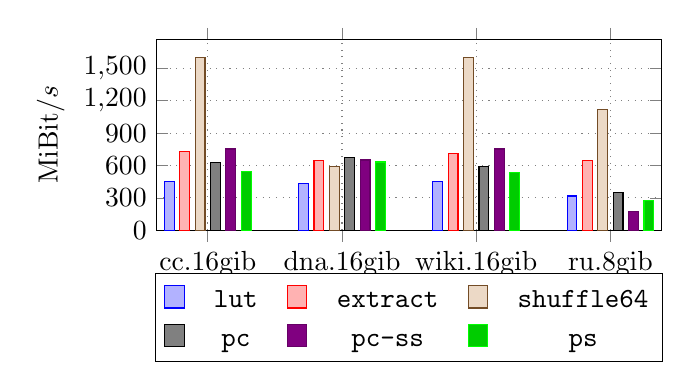
\begin{tikzpicture}
    \begin{axis} [
        width = 8cm,
        height = 4cm,
        ybar,
        bar width = 0.125cm,
        enlarge x limits = 0.1275,
        ylabel = $\text{MiBit}/s$,
        legend style = { 
            at = {(0.5, -0.225)},
            anchor = north,
            legend columns = 3,
            column sep = 2ex
        },
        ytick distance = 300,
        symbolic x coords = {
            % dblp.xml,
            % dna,
            % english,
            % pitches,
            % proteins,
            % sources,
            % chr22.dna,
            % etext99,
            % gcc-3.0.tar,
            % howto,
            % jdk13c,
            % linux-2.4.5.tar,
            % rctail96,
            % rfc,
            % sprot34.dat,
            % w3c2,
            cc.16gib,
            dna.16gib,
            wiki.16gib,
            ru.8gib
        }
    ]
    


        %% MULTIPLOT(type) SELECT file AS x, MEDIAN((height * (size / CAST(time_in_s AS Float))) / (1024 * 1024)) AS y,MULTIPLOT
        %% FROM stats WHERE (type LIKE 'lwt%' OR type LIKE '%tree') GROUP BY MULTIPLOT,x ORDER BY ds_order,MULTIPLOT,x
        \addplot coordinates { (cc.16gib,453.967) (dna.16gib,436.887) (ru.8gib,317.195) (wiki.16gib,447.952) };
        \addlegendentry{type=lwt-lut-16-4-4};
        \addplot coordinates { (cc.16gib,729.58) (dna.16gib,644.08) (ru.8gib,642.511) (wiki.16gib,714.417) };
        \addlegendentry{type=lwt-pext-16-4};
        \addplot coordinates { (cc.16gib,1604.84) (dna.16gib,593.957) (ru.8gib,1121.03) (wiki.16gib,1604.39) };
        \addlegendentry{type=lwt-shuffle-64-8};
        \addplot coordinates { (cc.16gib,628.456) (dna.16gib,669.698) (ru.8gib,346.956) (wiki.16gib,591.013) };
        \addlegendentry{type=pwm-pc-tree};
        \addplot coordinates { (cc.16gib,752.967) (dna.16gib,650.334) (ru.8gib,170.439) (wiki.16gib,753.049) };
        \addlegendentry{type=pwm-pc-ss-tree};
        \addplot coordinates { (cc.16gib,545.858) (dna.16gib,632.202) (ru.8gib,277.692) (wiki.16gib,535.149) };
        \addlegendentry{type=pwm-ps-tree};



        \legend {
            \texttt{lut}\strut,
            \texttt{extract}\strut,
            %\texttt{shuffle8}\strut,
            %\texttt{shuffle16}\strut,
            %\texttt{shuffle32}\strut,
            \texttt{shuffle64}\strut,
            \texttt{pc}\strut,
            \texttt{pc-ss}\strut,
            \texttt{ps}\strut
        }
        


    \end{axis}
\end{tikzpicture}
\end{frame}

\begin{frame}
    \frametitle{Ergebnisse (Wavelet Matrix)}
    \centering
    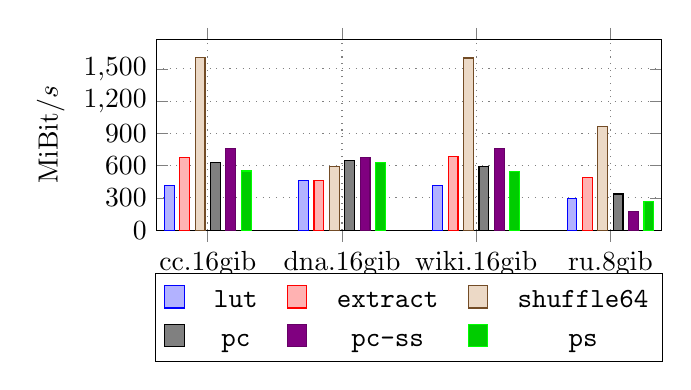
\begin{tikzpicture}
        \begin{axis} [
            width = 8cm,
            height = 4cm,
            ybar,
            bar width = 0.125cm,
            enlarge x limits = 0.1275,
            ylabel = $\text{MiBit}/s$,
            legend style = { 
                at = {(0.5, -0.225)},
                anchor = north,
                legend columns = 3,
                column sep = 2ex
            },
            ytick distance = 300,
            symbolic x coords = {
                % dblp.xml,
                % dna,
                % english,
                % pitches,
                % proteins,
                % sources,
                % chr22.dna,
                % etext99,
                % gcc-3.0.tar,
                % howto,
                % jdk13c,
                % linux-2.4.5.tar,
                % rctail96,
                % rfc,
                % sprot34.dat,
                % w3c2,
                cc.16gib,
                dna.16gib,
                wiki.16gib,
                ru.8gib
            }
        ]
        
    
    
            %% MULTIPLOT(type) SELECT file AS x, MEDIAN((height * (size / CAST(time_in_s AS Float))) / (1024 * 1024)) AS y,MULTIPLOT
            %% FROM stats WHERE (type LIKE 'wm%' OR type LIKE '%matrix') GROUP BY MULTIPLOT,x ORDER BY ds_order,MULTIPLOT,x
            \addplot coordinates { (cc.16gib,419.24) (dna.16gib,464.852) (ru.8gib,298.809) (wiki.16gib,417.959) };
            \addlegendentry{type=wm-lut-16-4-4};
            \addplot coordinates { (cc.16gib,677.655) (dna.16gib,461.728) (ru.8gib,489.259) (wiki.16gib,681.495) };
            \addlegendentry{type=wm-pext-8-8};
            \addplot coordinates { (cc.16gib,1610.08) (dna.16gib,594.277) (ru.8gib,968.329) (wiki.16gib,1600.97) };
            \addlegendentry{type=wm-shuffle-64-8};
            \addplot coordinates { (cc.16gib,625.573) (dna.16gib,651.686) (ru.8gib,336.96) (wiki.16gib,588.448) };
            \addlegendentry{type=pwm-pc-matrix};
            \addplot coordinates { (cc.16gib,757.9) (dna.16gib,674.329) (ru.8gib,169.981) (wiki.16gib,757.642) };
            \addlegendentry{type=pwm-pc-ss-matrix};
            \addplot coordinates { (cc.16gib,550.256) (dna.16gib,633.351) (ru.8gib,270.279) (wiki.16gib,542.189) };
            \addlegendentry{type=pwm-ps-matrix};
    
    
    
            \legend {
                \texttt{lut}\strut,
                \texttt{extract}\strut,
                %\texttt{shuffle8}\strut,
                %\texttt{shuffle16}\strut,
                %\texttt{shuffle32}\strut,
                \texttt{shuffle64}\strut,
                \texttt{pc}\strut,
                \texttt{pc-ss}\strut,
                \texttt{ps}\strut
            }
            
    
    
        \end{axis}
    \end{tikzpicture}
    \end{frame}


\end{document}


